\documentclass[twoside,10pt,a4paper]{article}
\usepackage[utf8]{inputenc}
\usepackage[english]{babel}
\usepackage{amsmath}
\usepackage{amsfonts}
\usepackage{amssymb}
\usepackage{graphicx}

\usepackage[left=2cm,right=2cm,top=2cm,bottom=3cm]{geometry}
\usepackage{fancyvrb}
\usepackage{listings}
\usepackage{xparse}
\usepackage{tikz} % ajout de dessins LaTeX
\usepackage{graphicx}
\usepackage{float}  % alignement des figures
\usepackage{fancyhdr}
\usepackage{enumitem}
\usepackage{verbatim}
\usepackage{xcolor}

\usepackage{caption}
\usepackage{subcaption}

\pagestyle{fancy} %fancyhdr
	\fancyhf{} %fancyhdr
	\renewcommand{\sectionmark}[1]{\markboth{#1}{}}
	\fancyhead[R]{NLDCI Set 5 Questions} %INSERT TITLE HERE FOR fancyhdr
	\fancyhead[L]{\nouppercase{\leftmark}} %fancyhdr
	\cfoot{\thepage} %fancyhdr
	\setlength{\headheight}{35pt}
	\setlength{\parindent}{0pt}
	
	\definecolor{MyBlue}{HTML}{4A90E2}
	\definecolor{MyRed}{HTML}{D0021B}
	\definecolor{MyGreen}{HTML}{7ED321} % Same color use in Mathcha

\begin{titlepage}
\title{\huge \textbf{Nonlinear Dynamics \& Chaos I \\ \Large Exercice Set 5 Questions}}	%TITLE
\author{ }		%AUTHOR
\date{ }	%DATE

\end{titlepage}


\begin{document}

\maketitle

\section*{Question 1}
Consider the quadratic \textit{Duffing equation}
\begin{align*}
	\dot{u} &= v, \\
	\dot{v} &= \beta u - u^2 - \delta v,
\end{align*}
where $\delta > 0$, and $0 \leq |\beta| \ll 1$.

\begin{enumerate}[label=(\alph*)]
	\item Construct a $\beta$-dependent center manifold up to quadratic order near the origin for small $\beta$ values.
	\item Construct a stability diagram for the reduced system on the center manifold using $\beta$ as a bifurcation parameter.
\end{enumerate}


\section*{Question 2}
Assume that a dynamical system, depending on a parameter $\mu$, undergoes a \underline{subcritical} Hopf bifurcation at $\mu = 0$. Let
\begin{equation*}
	\begin{cases}
		\dot{r} = r(d_0 \mu + a_0 r^2) \\
		\dot{\theta} = \omega + e_0 r^2 + b_0 \mu
	\end{cases}
\end{equation*}
be the truncated normal form on the center manifold $W_\mu^c$ in polar coordinates. Which figure represents the correct bifurcation diagram for this system?

\begin{enumerate}[label=(\alph*)]
	\item 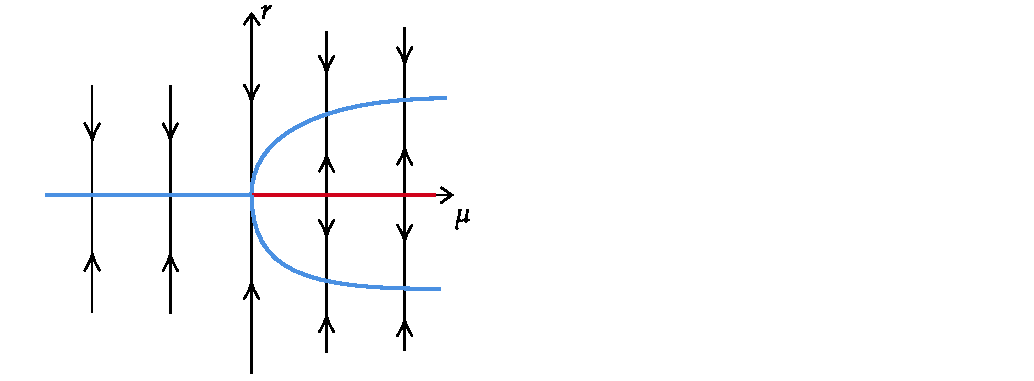
\includegraphics[scale=0.8]{Graphics/MCQ1_figures/Q14D01.pdf}
	\newpage
	\item 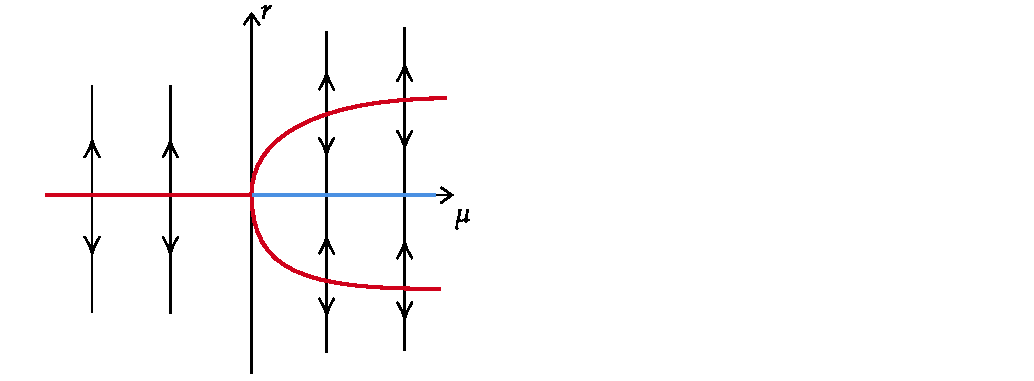
\includegraphics[scale=0.8]{Graphics/MCQ1_figures/Q14D02.pdf}
	\item 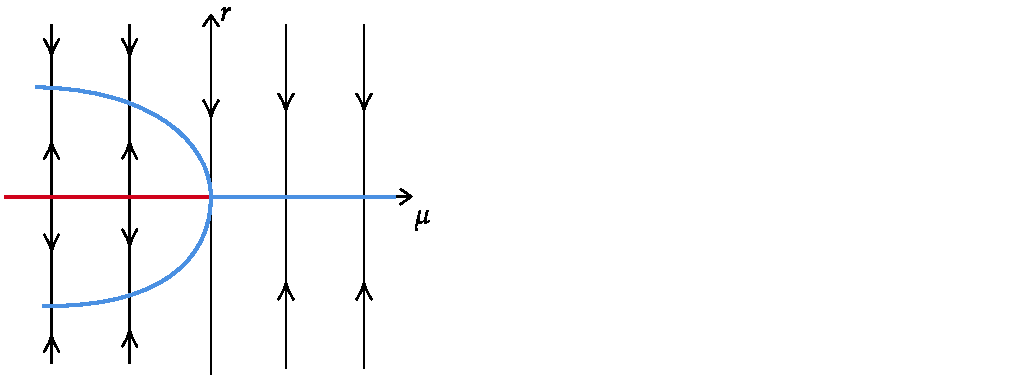
\includegraphics[scale=0.8]{Graphics/MCQ1_figures/Q14D03.pdf}
	\item 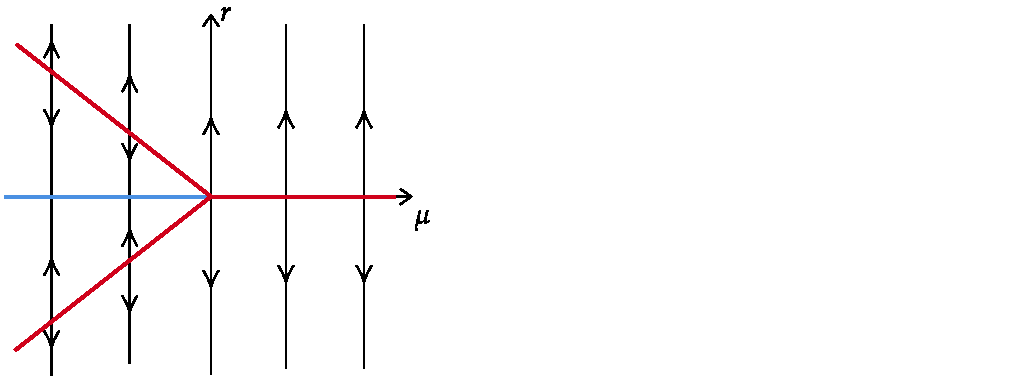
\includegraphics[scale=0.8]{Graphics/MCQ1_figures/Q14D04.pdf}
\end{enumerate}

\section*{Question 3}
Assume that the dynamical system $\dot{\mathbf{x}} = f(\mathbf{x}, \mu), \; (\mathbf{x} \in \mathbb{R}, \; \mu \in \mathbb{R})$ undergoes a codimension 1 bifurcation at $y = 0$. If $f(-x, \mu) = -f(x, \mu)$, what type of bifurcation is possible at $\mu = 0$?

\begin{enumerate}[label=(\alph*)]
	\item Saddle-node
	\item Transcritical
	\item Pitchfork
	\item None
\end{enumerate}

\newpage

\section*{Question 4}
Consider the dynamical system
\begin{equation*}
	\dot{x} = A(\mu)x + f(x;\mu)
\end{equation*}
where $ x \in \mathbb{R}, \; f(x,0) = -f(-x,0),\; \forall x \in \mathbb{R}, \; \mu \in \mathbb{R}, \; f\in C^1 $. Which of the following statements are true?

\begin{enumerate}[label=(\alph*)]
	\item This system cannot have a saddle-node bifurcation at $\mu = 0$.
	\item This system will have either a Hopf bifurcation or a transcritical bifurcation at $\mu = 0$.
	\item This system has a hyperbolic fixed point at $x = 0$, and hence cannot have a bifurcation at $\mu = 0$.
	\item None of the above
\end{enumerate}

\section*{Question 5}
Consider a dynamical system
\begin{equation*}
	\dot{x} = A(\mu^2)x + f(x, \mu)
\end{equation*}
where $x \in \mathbb{R}^2,\; A\in \mathbb{R}^{2 \times 2}, \; \mu \in \mathbb{R}, \; f(x, \mu) = \mathcal{O}(|x|^2), \; \nabla \cdot f(x) < 0$ for $|x| \ll 1$ where the $2 \times 2$ matrix depends on $\mu^2$. Assume that A(0) has a purely imaginary pair of eigenvalues.

Which of the following statements are true?

\begin{enumerate}[label=(\alph*)]
	\item This system has a subcritical Hopf bifurcation at $\mu = 0$.
	\item This system has a supercritical Hopf bifurcation at $\mu = 0$.
	\item The $x = 0$ fixed point does not undergo a Hopf bifurcation.
	\item The $x = 0$ fixed point undergoes a Hopf bifurcation, but its type cannot be determined from the information given.
\end{enumerate}


\end{document}